This section contains the preliminary experiments conducted on the proposed study. Specifically, this includes the two versions of the proposed model's results. The first version is the use of EfficientNetB0 and the second version is the use of the EfficientNetB1 base model. Each model has a different composition of the proposed model. The version that uses the EfficientNetB0 base model follows the initial proposed model defined in \ref{fig:initproposedmodel} we will call it Version 1 here, while the version that utilizes the EfficientNetB1 follows the \ref{fig:proposedmodel} we will call it Version 2. The reason why there are two versions is because of the improvement on the model in the later time than the conduct of some experiments. Some tests are not included here because they were done to correct the implementation of accessing of dataset and color space conversion, model improvements, consistency check for the siamese model, and transitional improvement from CNN to SCNN. 

\begin{figure}[h]
	\centering
	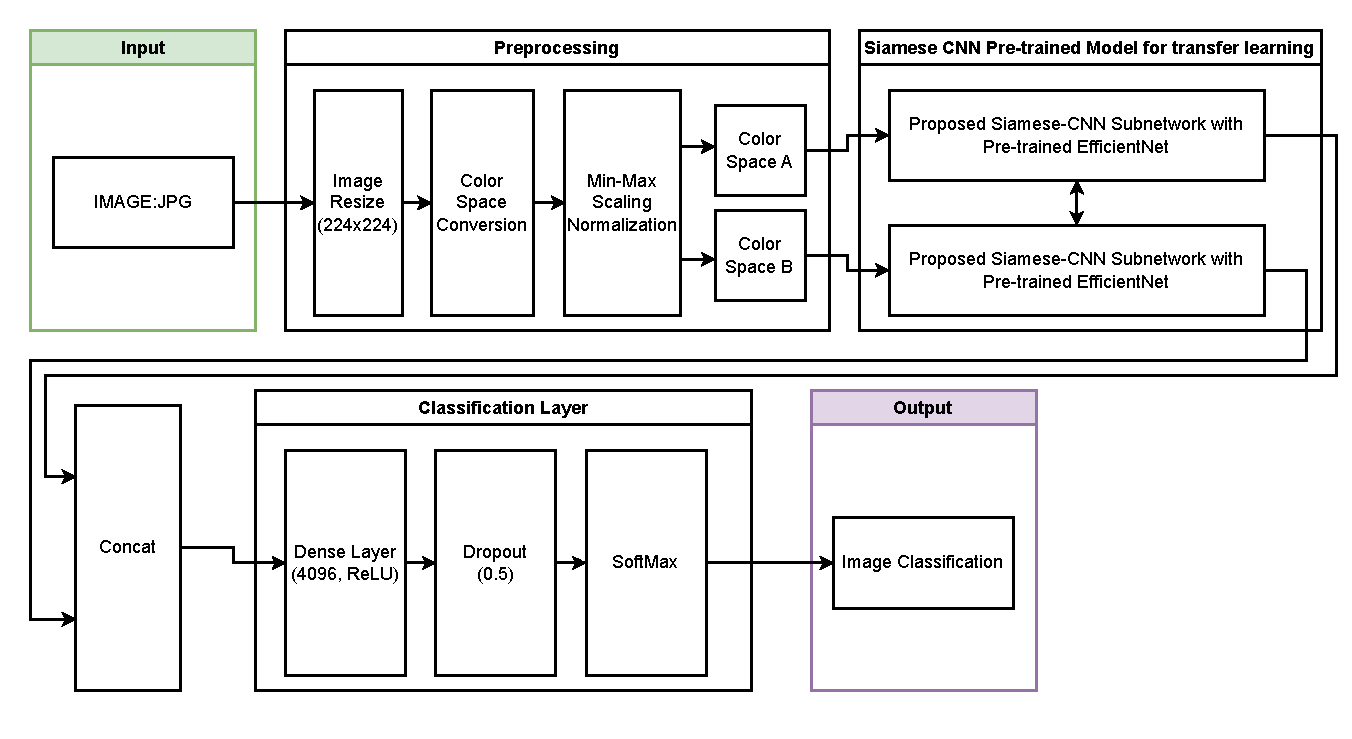
\includegraphics[width=1.0\textwidth]{graphics/images/Proposed_Model-old.pdf}
	\caption{Initial FoodWhizNet Framework}
	\label{fig:initproposedmodel}
\end{figure}

\section{Version 1 Experiments}
As mentioned earlier, Version 1 utilized the initial proposed model shown in \ref{fig:initproposedmodel} with the EfficientNetB0 base model. This particular experiment tests the best two-color space combination. Specifically, the combination of RGB and the other 10 color spaces.
\subsection{Dataset}
The conduct of this experiment includes the use of the Food101 dataset with 14 classes as identified in \cite{kaur-2023} which achieved an accuracy of 87.7\% using the EfficientNetB0 model on CNN with default RGB image. Table \ref{tab:f101c14} shows the 14 classes included in the experiment.

\begin{table}[htbp]
  \centering
  \begin{tabular}{|c|c|}
    \hline
    \textbf{Class Number} & \textbf{Class Name} \\
    \hline
    1 & apple\_pie \\
    2 & bread\_pudding \\
    3 & breakfast\_burrito \\
    4 & chicken\_wings \\
    5 & eggs\_benedicts \\
    6 & fish\_and\_chips \\
    7 & french\_fries \\
    8 & french\_onion\_soup \\
    9 & french\_toast \\
    10 & fried\_rice \\
    11 & grilled\_cheese\_sandwich \\
    12 & pizza \\
    13 & pulled\_pork\_sandwich \\
    14 & spring\_rolls \\
    \hline
  \end{tabular}
  \caption{Food 101 with 14 Classes}
  \label{tab:f101c14}
\end{table}

\subsection{Configuration}
Additional configuration includes a EarlyStopping callback with patience of 7 and monitoring the validation loss. LowerLROnPlateau callback also monitors the validation loss and a patience of 5. This experiment is a fine-tuning.
\begin{table}[htbp]
  \centering
  \begin{tabular}{|c|c|}
    \hline
    \textbf{[Hyper]parameter} & \textbf{Value} \\
    \hline
    Optimizer & Adam with initial LR of 0.01 \\
    Epochs & 100 \\
    Loss Function & Categorical Crossentropy \\
    Batch Size & 32 \\
    Shuffle Buffer Size & 1000 \\
    Shuffle Seed & 20 \\
    Augmentation Layer Seed & 42 \\
    Augmentation Layer Factors & 0.2 \\
    SubNetwork Dropout & 30\% \\
    Classification Dropout & 50\% \\
    \hline
  \end{tabular}
  \caption{Experiment Configuration of Version 1}
  \label{tab:config-v1}
\end{table}

\subsection{Results}
In this experiment of finding the best two-color space combination, RGB and XYZ stands out among the rest of the RGB combinations. Garnering a 75.51\% Top 1\% accuracy, that is 5.58\% higher than the second highest. It also achieved the top score in the Top 5\% and the lowest final loss. It has also had a promising run where it found its best weights in the 23rd epoch.
\begin{table}[h]
  \centering
  \resizebox{\textwidth}{!} & \textbf{Final Top 1\%} & \textbf{Epochs} & \textbf{Best Epoch} \\
    \hline
    RGB+LAB & 1.056701 & 94.2571 & 66.4000 &37 &27\\
    RGB+HSV & 1.120901 &92.1714 & 65.6286 & 34 & 27 \\
    RGB+HED & 1.328380 &90.1429&59.1143&31&24 \\
    RGB+LUV & 1.046469 &93.6000&67.0000&41&34 \\
   \textbf{ RGB+XYZ} & \textbf{0.816763} &\textbf{95.6571}&\textbf{75.5143}&30&23 \\
    RGB+YCbCr & 1.009330&93.4571&69.6571&41&34 \\
    RGB+YIQ &1.110264 &93.5714&65.4571&28&21 \\
    RGB+YDbDr &0.989937 &94.1714&69.8000&28&21 \\
    RGB+YPbPr & 1.057165&92.9429&67.9429&41&34\\
    RGB+YUV &1.172660 &91.4000&62.3714&28&21 \\
    \hline
  \end{tabular}
   }
  \caption{Color Space combination Results}
  \label{tab:cscr}
\end{table}

\section{Version 2 Experiment}
Version 2 utilized the new proposed model developed from model improvement to handle a large number of classes. Since the Version 1 experiment exhibits poor results on 14 classes of food 101, it might struggle to achieve even the minimum with the whole 101 classes of Food 101. It can also be observed that on \cite{kaur-2023}, they got 87.7\% for the 14 classes and the initial proposed model is far from that state-of-the-art. 

\subsection{Dataset}
The dataset used is the whole Food101 dataset \cite{bossard-2014} and profiled in table \ref{tab:dataprofile}. 

\subsection{Configuration}
The configuration includes a EarlyStopping callback with patience of 3 and monitoring the validation accuracy. LowerLROnPlateau callback also monitors the validation accuracy and a patience of 0. This experiment is a fine-tuning.

\begin{table}[htbp]
  \centering
  \begin{tabular}{|c|c|}
    \hline
    \textbf{[Hyper]parameter} & \textbf{Value} \\
    \hline
    Optimizer & Adam with initial LR of 0.01 \\
    Epochs & 100 \\
    Loss Function & Categorical Crossentropy \\
    Batch Size & 32 \\
    Shuffle Buffer Size & 1000 \\
    Shuffle Seed & 20 \\
    Augmentation Layer Seed & 42 \\
    Augmentation Layer Factors & 0.2 \\
    SubNetwork Dropout & 30\% \\
    Classification Dropout & 40\% \\
    \hline
  \end{tabular}
  \caption{Experiment Configuration of Version 2}
  \label{tab:config-v2}
\end{table}
\subsection{Results: RGB+LAB}
This version utilized the EfficientNetB1 base model. The structure of the model can be seen in \ref{fig:proposedmodel}. Ran using the RGB and LAB combination, the results are shown in figure \ref{fig:v2-accu1} for the Top 1\% accuracy of the new model with 69.93\%, \ref{fig:v2-accu5} for the Top 5\% with 90.18\%, and figure \ref{fig:v2-loss} for the final loss with 1.2020. The training took 17 epochs in total and the best weight was found on epoch 14.

\begin{figure}[htbp]
  \centering

  \begin{subfigure}[b]{0.45\textwidth}
    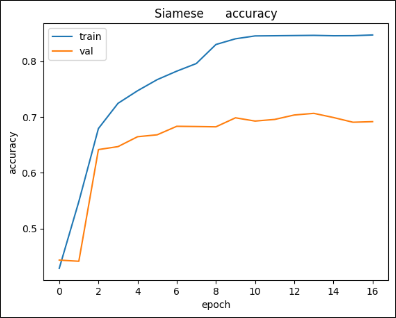
\includegraphics[width=\textwidth]{graphics/images/results/v2-accu1.png}
    \caption{Top 1 Accuracy RGB+LAB}
    \label{fig:v2-accu1}
  \end{subfigure}
  \hfill
  \begin{subfigure}[b]{0.45\textwidth}
    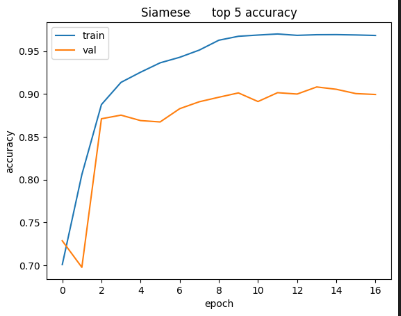
\includegraphics[width=\textwidth]{graphics/images/results/v2-accu5.png}
    \caption{Top 5 Accuracy RGB+LAB}
    \label{fig:v2-accu5}
  \end{subfigure}
  \medskip
  \begin{subfigure}[b]{0.45\textwidth}
    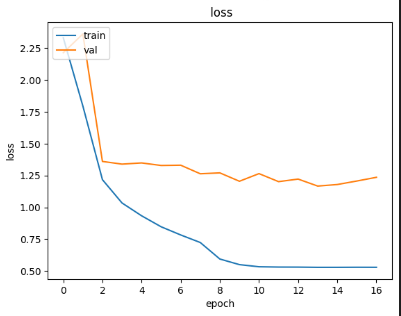
\includegraphics[width=\textwidth]{graphics/images/results/v2-loss.png}
    \caption{Final Loss RGB+LAB}
    \label{fig:v2-loss}
  \end{subfigure}
  \caption{FoodWhizNet Model Results for RGB+LAB}
  \label{fig:fwnresults}
\end{figure}

\subsection{Results: RGB+XYZ}
The same setup as the RGB+LAB experiment of Version 2, the RGB+XYZ experiment was conducted based on the initial result from the Version 1 experiment. The results are shown in figure \ref{fig:v2-accu1-rgbxyz} for the Top 1\% accuracy with 80.07\%, \ref{fig:v2-accu5-rgbxyz} for the Top 5\% with 95.04\%, and figure \ref{fig:v2-loss-rgbxyz} for the final loss with 0.7663. The training took 13 epochs in total and the best weight was found on epoch 10.

\begin{figure}[htbp]
  \centering

  \begin{subfigure}[b]{0.45\textwidth}
    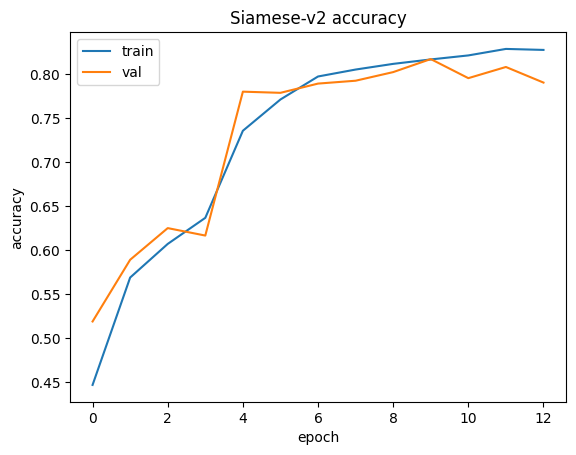
\includegraphics[width=\textwidth]{graphics/images/results/v2-accu1-rgbxyz.png}
    \caption{Top 1 Accuracy RGB+XYZ}
    \label{fig:v2-accu1-rgbxyz}
  \end{subfigure}
  \hfill
  \begin{subfigure}[b]{0.45\textwidth}
    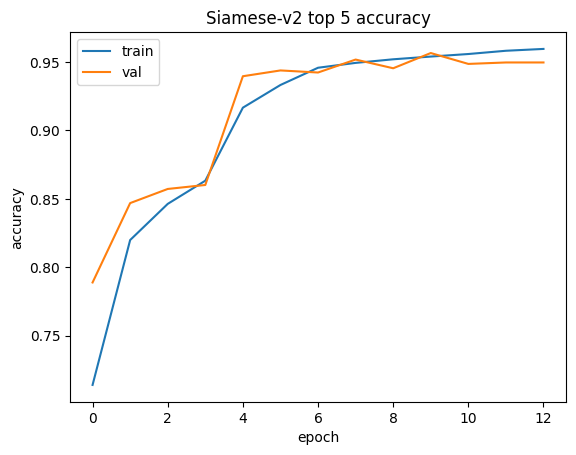
\includegraphics[width=\textwidth]{graphics/images/results/v2-accu5-rgbxyz.png}
    \caption{Top 5 Accuracy RGB+XYZ}
    \label{fig:v2-accu5-rgbxyz}
  \end{subfigure}
  \medskip
  \begin{subfigure}[b]{0.45\textwidth}
    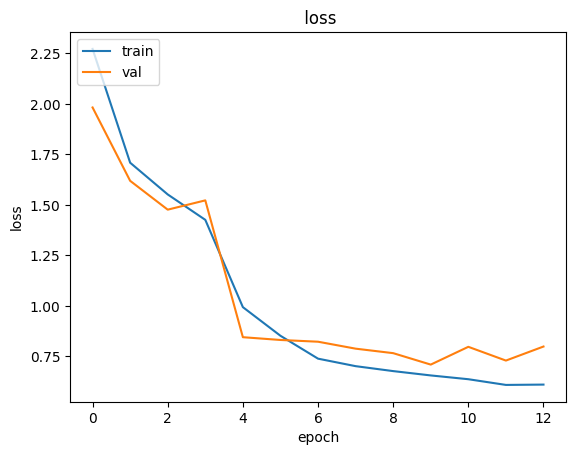
\includegraphics[width=\textwidth]{graphics/images/results/v2-loss-rgbxyz.png}
    \caption{Final Loss RGB+XYZ}
    \label{fig:v2-loss-rgbxyz}
  \end{subfigure}
  \caption{FoodWhizNet Model Results for RGB+XYZ}
  \label{fig:fwnresultsrgbxyz}
\end{figure}